\section{Peano-Jordan Measure}

In this chapter, we aim to provide a definition of the \emph{measure} of a
subset $E\subset \RR^n$, formalizing the same notions that were essentially
already used by the ancient Greeks. We will do this in the case most relevant to
us, namely the planar case $n=2$, where the \emph{measure} of a set is called
\emph{area}. However, the entire construction could be carried out without any
difficulty (except for the notations becoming more complex) in the general case
of dimension $n$.

Given a set $E\subset \RR^2$, we wish to define its area $m(E)\in \RR$ in such a
way that the following properties hold:
\begin{enumerate}
  \item if $E\cap F=\emptyset$, then $m(E\cup F) = m(E) + m(F)$ (additivity);
  \item if $E \subset F$, then $m(E) \le m(F)$ (monotonicity);
  \item if $E=[x_1,x_2]\times [y_1,y_2]$, then $m(E) = \abs {x_2-x_1}\cdot \abs{y_2-y_1}$ (normalization).
\end{enumerate}

We will define the measure $m$ on a family of subsets of $\RR^2$ that we will
call \emph{Peano-Jordan measurable}. It could be demonstrated that it is not
possible to define $m$ on all subsets of $\RR^2$ in such a way that the
properties stated above hold. However, it would be possible to define the
measure on a much broader class of sets than those we will consider, by imposing
additivity not only on finite unions but also on countable unions
($\sigma$-additivity). What would be obtained is the so-called \emph{Lebesgue}
measure, which is now a standard construction in mathematical analysis but would
require a much more complex theory to develop. Here, we will be content to
introduce the Peano-Jordan measure $m$ (finitely additive measure), which will
then allow us to give geometric meaning to the Riemann integral.
\index{measure!Peano-Jordan}%
\index{Peano-Jordan!measure of}%
\index{additive!measure}%

We will say that a set $R\subset \RR^2$ is a \emph{Cartesian rectangle}%
\mymargin{Cartesian rectangle}%
\index{rectangle!Cartesian}
if $R$ is the Cartesian product of two bounded intervals, that is,
\[
  R = I\times J
\]
with $x_1=\inf I>-\infty$,
$x_2=\sup I<+\infty$,
$y_1=\inf J > -\infty$,
$y_2=\sup J < +\infty$.

If $I=[x_1,x_2]$ and $J=[y_1,y_2]$, then, in order for the normalization
property to hold, we must set:
\[
  m([x_1,x_2]\times[y_1,y_2]) = \abs{x_2-x_1}\cdot\abs{y_2-y_1}.
\]

If $I=(x_1,x_2)$ and $J=(y_1,y_2)$ are open (and bounded) intervals, then for
every $\eps>0$ with $\eps<(x_2-x_1)/2$ and $\eps<(y_2-y_1)/2$, we have
\[
  [x_1+\eps,x_2-\eps] \times [y_1+\eps,y_2-\eps]
  \subset (x_1,x_2)\times (y_1,y_2)
  \subset [x_1,x_2]\times [y_1,y_2]
\]
from which, in order for the monotonicity property to hold, we must have:
\[
    (x_2-x_1-2\eps)\cdot (y_2-y_1-2\eps) \le m((x_1,x_2)\times(y_1,y_2)) \le
  \abs{x_2-x_1}\cdot \abs{y_2-y_1}.
\]
But for this to be true for every $\eps>0$, we must necessarily set:
\[
  m((x_1,x_2)\times(y_1,y_2)) = \abs{x_2-x_1}\cdot\abs{y_2-y_1}.
\]
The same holds if the intervals are semi-open or if we consider any set $E$ such
that $(x_1,x_2)\times (y_1,y_2) \subset E \subset [x_1,x_2]\times[y_1,y_2]$.
Thus, the area of a rectangle does not change if we add or remove points from
its sides.

If a set $E\subset \RR^2$ can be written as a finite union of disjoint
rectangles:
\[
  E = R_1 \cup R_2 \cup \dots \cup R_N
  \qquad
  R_i \cap R_j=\emptyset\text{ if } i\neq j
\]
we will say that $E$ is a \emph{Cartesian polyrectangle}%
\mymargin{Cartesian polyrectangle}%
\index{polyrectangle!Cartesian}.
In such a case, to ensure the additivity of the area, we will set:
\[
  m(E) = m(R_1) + \dots + m(R_N).
\]
For this to be a good definition, we must verify that if $A$ can be written as a
union of disjoint rectangles in two different ways, then the sum of the measures
of the rectangles gives the same result with both decompositions. This is
intuitively obvious and depends on the fact that given two different
decompositions into rectangles, it is possible to consider a grid formed by all
the lines containing the sides of each rectangle. This grid identifies a
decomposition into small rectangles that can be used to reconstruct both
decompositions. Each rectangle in the two decompositions will be a union of
small rectangles, and its area will be the sum of the areas of the small
rectangles. But since the two decompositions are subdivided into the same small
rectangles, the areas defined by the two decompositions must coincide.

\begin{figure}
  \hfill
  \subcaptionbox{}
  {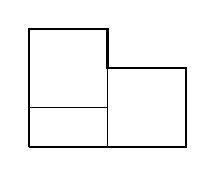
\begin{tikzpicture}[x=0.5cm, y=0.5cm]
      \draw[thick] (1,1) -- (5,1) -- (5,3) -- (3,3) -- (3,4) -- (1,4) -- (1,1);
      \draw (1,2) -- (3,2);
      \draw (3,1) -- (3,3);
  \end{tikzpicture}}
  \hfill
  \subcaptionbox{}
  {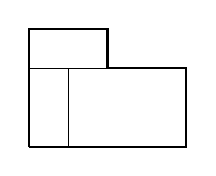
\begin{tikzpicture}[x=0.5cm, y=0.5cm]
      \draw[thick] (1,1) -- (5,1) -- (5,3) -- (3,3) -- (3,4) -- (1,4) -- (1,1);
      \draw (1,3) -- (3,3);
      \draw (2,1) -- (2,3);
  \end{tikzpicture}}
  \hfill
  \subcaptionbox{}
  {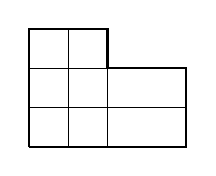
\begin{tikzpicture}[x=0.5cm, y=0.5cm]
      \draw[thick] (1,1) -- (5,1) -- (5,3) -- (3,3) -- (3,4) -- (1,4) -- (1,1);
      \draw (1,2) -- (5,2);
      \draw (1,3) -- (3,3);
      \draw (2,1) -- (2,4);
      \draw (3,1) -- (3,4);
  \end{tikzpicture}}
  \hfill\mbox{}
  \caption{The same polyrectangle can be obtained as two different unions of rectangles: (a), (b). Considering all the lines containing the sides of all the rectangles involved results in a subdivision (c) where each rectangle in (a) or (b) is a union of rectangles in (c).}
\end{figure}

For the same reason, it is clear that if $E$ and $F$ are two polyrectangles,
then $E\cup F$, $E \cap F$, $E\setminus F$, and $F\setminus E$ are also
polyrectangles, and it holds that
\begin{equation}\label{eq:48474624}
  m(E \cup F) = m(E\setminus F) + m(E\cap F) + m(F\setminus E).
\end{equation}
Indeed, it is possible to find a family of small rectangles (those identified by
the grid of all the lines containing the sides of the rectangles of $E$ and the
rectangles of $F$) that are disjoint from each other and such that $E\cap F$,
$E\setminus F$, and $F\setminus E$ can be written as unions of these small
rectangles. These sets are disjoint from each other, and therefore, by writing
the area of each as the sum of the areas of the rectangles, we
find~\eqref{eq:48474624}.

If we now take any set $E\subset \RR^2$ and impose that the monotonicity
property holds, we must have that $m(E)$, if it is definable, must be the
separating element between the measures of the polyrectangles contained in $E$
and those containing $E$. This justifies the following.

\begin{definition}[Peano-Jordan measure]
\label{def:peano-jordan}%
\mymargin{Peano-Jordan}%
\index{Peano-Jordan}%
\index{measure!Peano-Jordan}%
\index{Peano-Jordan!measure of}%
\index{Jordan!measure of}%
Let $E\subset \RR^2$ be a bounded set. We define:
\begin{align*}
m^*(E) &= \inf\ENCLOSE{m(F)\colon \text{$F\supset E$, $F$ polyrectangle}}, \\
m_*(E) &= \sup\ENCLOSE{m(F)\colon \text{$F\subset E$, $F$ polyrectangle}}.
\end{align*}

Since $E$ is bounded (thus contained in a bounded rectangle), we have
$m^*(E)<+\infty$, and since $\emptyset \subset E$ and $m(\emptyset)=0$ (the
empty set $\emptyset = (a,a) \times (c,c)$ is a polyrectangle of zero area), we
have $m_*(E)\ge 0$. Moreover, $m_*(E)\le m^*(E)$ because every polyrectangle
contained in $E$ is contained, and therefore has an area not greater than, any
polyrectangle containing $E$.

If $m^*(E) = m_*(E)$, we say that $E$ is \emph{measurable}%
\mymargin{measurable}%
\index{measurable} according to Peano-Jordan and set $m(E) = m^*(E) = m_*(E)$ as its Peano-Jordan measure.
\end{definition}

\begin{theorem}[properties of the Peano-Jordan measure]
If $E$ and $F$ are Peano-Jordan measurable, then $E\cup F$, $E\setminus F$,
$F\setminus E$, and $E\cap F$ are also Peano-Jordan measurable, and it holds
that
\begin{align*}
  m(E\cup F)
  &= m(E\setminus F) + m(E\cap F) + m(F\setminus E)\\
  &= m(E) + m(F) - m(E\cap F).
\end{align*}
\end{theorem}
%
\begin{proof}
We observe that a set $E$ is measurable if and only if for every $\eps>0$, there
exist polyrectangles $E_*, E^*$ with $E_* \subset E \subset E^*$ such that
$m(E^*)-m(E_*)<\eps$ (this follows from the characterization of supremum and
infimum).

\begin{figure}
  \centering\input{figures/figurePJ}
  \caption{The sets $E$ and $F$ and the approximating polyrectangles from the inside and outside. The approximations can be chosen so that the frame between the external and internal polyrectangles has an area smaller than any $\eps>0$.}
  \label{fig:PeanoJordan}
\end{figure}
Thus, under our assumptions, for every $\eps>0$, there exist polyrectangles
$E^*$, $E_*$, $F^*$, $F_*$ such that
\[
   E_* \subset E \subset E^*, \qquad
   F_* \subset F \subset F^*
\]
with
\[
  m(E^*)-m(E_*) < \eps,\qquad
  m(F^*)-m(F_*) < \eps.
\]
We can then approximate the sets $E\cap F$, $E\cup F$, and $E\setminus F$ from
the inside and outside with polyrectangles:
\begin{gather*}
  E_*\cap F_* \subset E\cap F \subset E^*\cap F^*, \\
  E_*\cup F_* \subset E\cup F \subset E^* \cup F^*, \\
  E_* \setminus F^* \subset E\setminus F \subset E^*\setminus F_*.
\end{gather*}
The differences between the external and internal approximations are always
contained in the union of the frames $\Delta = (E^*\setminus E_*)\cup
(F^*\setminus F_*)$ (refer to figure~\ref{fig:PeanoJordan}):
\begin{align*}
  (E^*\cap F^*) \setminus (E_* \cap F_*) \subset \Delta \\
  (E^*\cup F^*) \setminus (E_*\cup F_*) \subset \Delta \\
  (E^*\setminus F_*) \setminus (E_* \setminus F^*) \subset \Delta
\end{align*}
and thus, since $m(\Delta)<2\eps$ and since $\eps>0$ is arbitrary, we can
conclude that the sets $E\cap F$, $E\cup F$, and $E\setminus F$ are measurable.
With the same considerations, it can be easily verified that the union of the
disjoint polyrectangles $E_*\setminus F^*$ and $E_*\cap F_*$ differs from the
polyrectangle $E_*$ by a set of measure less than $\eps$, and thus, passing to
the limit as $\eps\to 0$, we obtain:
\[
  m(E\setminus F) + m(E\cap F) = m(E).
\]
By reversing the roles of $E$ and $F$, we obtain that $F\setminus E$ is also
measurable, and the analogous relation holds. With entirely similar
considerations, we obtain
\[
  m(E\cup F) = m(E) + m(F\setminus E).
\]
Consequently, the equalities stated in the theorem are obtained.
\end{proof}

\begin{theorem}[area element of a linear transformation]
\label{th:area_lineare}%
\index{element!of area}%
\index{measure!linear transformation}%
Let $E\subset \RR^2$ and let $L\colon \RR^2\to\RR^2$ be a linear affine
transformation:
\[
  L(x,y) = M\cdot \begin{pmatrix}
    x \\ y
  \end{pmatrix}
  + \begin{pmatrix}
    x_0 \\ y_0
  \end{pmatrix}
\]
with $M$ a $2\times 2$ matrix and $(x_0 ,y_0)\in \RR^2$.
Then if $E$ is Peano-Jordan measurable, $L(E)$ is also measurable. In such a
case, we have
\begin{equation}\label{eq:formula_area}
  m(L(E)) = \abs{\det M} \cdot m(E).
\end{equation}
\end{theorem}
%
\begin{proof}

We first observe that it is sufficient to verify what happens in the case where
$E$ is a Cartesian rectangle. Indeed, a generic measurable set $E$ can be
approximated, for every $\eps>0$, with polyrectangles $E^\pm$ with $E^-\subset E
\subset E^+$ and $m(E^+) - m(E^-) < \eps$. Suppose that $R^+_k$, for $k=1,\dots,
N^+$, are the rectangles composing $E^+$ and $R^-_k$, for $k=1,\dots, N^-$, are
the rectangles composing $E^-$. If we know that the transformation $L$ maps
rectangles into measurable sets and if we know that on Cartesian rectangles it
holds $m(L(R)) = c \cdot m(R)$, with $c= \abs{\det M}$, then it follows that
$L(R_k^+)$ can be approximated from the outside with a polyrectangle $F_k^+$
such that $m(F_k^+) - m(L(R_k^+)) < \eps/N^+$, while $L(R_k^-)$ can be
approximated from the inside with a polyrectangle $F_k^-$ such that
$m(L(R_k^-))-m(F_k^-) < \eps/N^-$. By taking the union $F^+ = F_1^+ \cup \dots
\cup F_{N^+}^+$ and $F^- = F_1^- \cup \dots \cup F_{N^-}^-$, we obtain
polyrectangles such that $F^- \subset L(E)\subset F^+$ and $m(F^+) - m(F^-) <
(c\cdot  m(E^+) + \eps) - (c \cdot m(E^-) -\eps) < (c+2) \eps$. Since $\eps>0$
is arbitrary, it follows that $L(E)$ is measurable and $m(L(E)) = c\cdot  m(E)$.

\emph{Step 1.}
Suppose that $L(x,y) = (\lambda x,\mu y)$ (a diagonal linear transformation). If
$E$ is a rectangle $E=[x_1,x_2]\times[y_1,y_2]$, then if $\lambda\ge 0$, $\mu\ge
0$, we have $L(E) = [\lambda x_1, \lambda x_2] \times [\mu y_1, \mu y_2]$, and
clearly $m(L(E)) = \lambda (x_2-x_1) \mu (y_2-y_1) = \lambda \mu m(E)$. Since
$\det L = \lambda \mu$, we have obtained the desired result. If $\lambda$ or
$\mu$ have a negative sign, the endpoints of the intervals can be swapped, and
in such a case, we obtain $m(L(E)) = \abs{\lambda}\abs{x_2-x_1} \cdot \abs{\mu}
\cdot \abs{y_2-y_1}$, and thus, as desired, $m(L(E))=\abs{\det L} \cdot m(E)$.

A possible translation component $(x_0,y_0)$ is irrelevant and will not be
considered further since translated rectangles maintain the same measure.

\emph{Step 2.}
Suppose that $L(x,y) = (y,x)$ (reflection with respect to the line $y=x$). This transformation has an associated matrix $M=\begin{pmatrix}0&1\\1&0\end{pmatrix}$ with determinant $-1$. Analytically, it swaps the coordinates $x$ and $y$. It is therefore immediate to verify that rectangles are mapped to rectangles with swapped base and height, and thus the Peano-Jordan measure (and measurability) remain unchanged. Therefore, the theorem is trivially valid in this case.

\begin{figure}
  {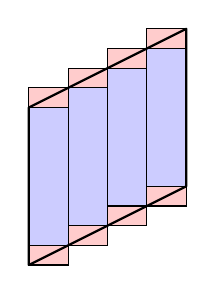
\begin{tikzpicture}[x=0.5cm, y=0.5cm]
    \draw[fill=red!20,draw=black] (0,0) -- (1,0) -- (1,0.5) -- (2,0.5) -- (2,1) -- (3,1) -- (3,1.5) -- (4,1.5) -- (4,6) 
        -- (3,6) -- (3,5.5) -- (2,5.5) -- (2,5) -- (1,5) -- (1,4.5) -- (0,4.5)
    -- cycle;
    \draw[fill=blue!20,draw=black] (0,0.5) -- (1,0.5) -- (1,1) -- (2,1) -- (2,1.5) -- (3,1.5) -- (3,2) -- (4,2) -- (4,5.5)
        -- (3,5.5) -- (3,5) -- (2,5) -- (2,4.5) -- (1,4.5) -- (1,4) -- (0,4) --
    cycle;
    \draw (1,1) -- (1,4);
    \draw (2,1.5) -- (2,4.5);
    \draw (3,2) -- (3,5);
    \draw[thick,line join=round] (0,0) -- (4,2) -- (4,6) -- (0,4) -- cycle;
  \end{tikzpicture}}
  \caption{Approximation of a parallelogram using Cartesian polyrectangles.}
\end{figure}

\emph{Step 3.}
Suppose that $E=[a,b]\times[c,d]$ and $L(x,v)=(x,rx+v)$ with $r\in \RR$ fixed
(we are using the coordinates $(x,v)$ in the domain of $L$ and the coordinates
$(x,y)$ in the codomain). Then
\[
  L(E) = \{(x,y)\in \RR^2\colon x\in[a,b], rx+c \le y \le rx+d\}
\]
is a parallelogram. Suppose, for the sake of argument, that $r\ge 0$. For every
$n\in \NN$, I can slice the set $L(E)$ with the vertical lines $x_k =
a+\frac{r}{n}(b-a)$ and identify the rectangles, for $k=1,\dots, n$:
\begin{align*}
   R_{k,n}^-
   &= \{(x,y)\in \RR^2 \colon x\in [x_{k-1},x_k), y\in[r x_k+c,r x_{k-1}+d]\},
   \\
   R_{k,n}^+
   &= \{(x,y)\in \RR^2 \colon x\in [x_{k-1},x_k), y\in[r x_{k-1}+c,r x_k+d]\}.
\end{align*}
and the polyrectangles obtained by combining these rectangles:
\begin{align*}
  P^-_n &= R_{1,n}^- \cup R_{2,n}^- \cup \dots \cup R_{n,n}^-, \\
  P^+_n & = R_{1,n}^+ \cup R_{2,n}^+ \cup \dots \cup R_{n,n}^+.
\end{align*}
By construction, we observe that
\[
  P^-_n \subset L(A) \subset P^+_n.
\]
But it is easy to calculate the measures of these polyrectangles:
\begin{align*}
  m(P^-_n) &= \sum_{k=1}^n m(R_{k,n}^-)
          = \sum_{k=1}^n(x_k-x_{k-1})\cdot (d-c-r(x_k-x_{k-1}))\\
         &= \sum_{k=1}^n \frac {b-a} n \cdot \enclose{d-c-\frac{r}{n}}
          = (b-a)\cdot \enclose{d-c-\frac{r}{n}} \\
    m(P^+) &= \sum_{k=1}^n m(R_{k,n}^+) = \dots = (b-a)\cdot
  \enclose{d-c+\frac{r}{n}}
\end{align*}
but since for $n\to +\infty$, we have $m(P^-_n)\to (b-a)\cdot(d-c)$ and
$m(P^+_n) \to (b-a)\cdot(d-c)$, and since we have
\[
  m(P^-_n)\le m_*(L(A))\le m^*(L(E)) \le m(P^+_n)
\]
we obtain that $L(E)$ is measurable and $m(L(E)) = (b-a)\cdot(d-c) = m(E)$. The matrix associated with $L$ is $M=\begin{pmatrix}1 & 0 \\ r & 1 \end{pmatrix}$, and thus $\det M = 1$. We have therefore found the desired result.

\emph{Step 4.}
Let $L$ be any linear transformation obtained as a composition of the
transformations considered earlier: $L= L_n\circ \dots  \circ L_2 \circ L_1$.
Then, from what has already been seen, we know that if $E$ is any Peano-Jordan
measurable set, it holds that
\[
m(L(E)) = m\enclose{L_n(\dots(L_2(L_1(E)))\dots)}
     = \abs{\det L_n} \cdots \abs{\det L_2} \cdot \abs{\det L_1} \cdot m(E)
\]
and thus $L(E)$ is also Peano-Jordan measurable, and since
\[
 \abs{\det L} = \abs{\det L_n} \cdots \abs{\det L_1}
\]
the formula~\eqref{eq:formula_area} is verified.

\emph{Step 5.}
To conclude the proof, it is therefore sufficient to verify that every linear
transformation can be written as a composition of the transformations already
considered. In general, the theorem can be formulated in any dimension (in
$\RR^n$ instead of $\RR^2$), and the proof proceeds in exactly the same way by
considering only transformations involving two coordinates. The transformation
that swaps two coordinates (step 2) is represented by a matrix that, if
multiplied on the left of a generic matrix $M$, swaps its rows, and if
multiplied on the right, swaps its columns. The transformation of step 3, if
applied on the left, adds a multiple of one row to another row, and if applied
on the right, adds a multiple of one column to another column. Through the
Gaussian elimination method (complete reduction), it is possible to transform
any matrix using only these transformations in such a way as to keep the modulus
of the determinant invariant and make the matrix diagonal. At that point, we
have reduced it to step 1.

In the planar case, $n=2$, we can explicitly perform Gaussian elimination.
Suppose that the linear transformation $L$ is associated with a generic matrix:
\[
  M = \begin{pmatrix} a&b\\c&d\end{pmatrix}.
\]
Without loss of generality, we can assume that $a\neq 0$ (if all elements were
zero, we would have $M=0$, which is already in diagonal form). Then we add a
multiple $r$ of the first row to the second row to eliminate the term $b$:
\[
\begin{pmatrix} 1&0\\r&1
\end{pmatrix}\cdot
    \begin{pmatrix} a&b\\c&d
    \end{pmatrix}
  =
  \begin{pmatrix} a&b\\c+ra&d+rb
  \end{pmatrix}
\]
choosing $r=-\frac c a$ and setting $d'=d+rb$, we obtain the matrix:
\[
\begin{pmatrix} a&b\\0&d'
\end{pmatrix}.
\]
Now observe that
\[
      \begin{pmatrix} 0&1\\1&0
      \end{pmatrix}\cdot
      \begin{pmatrix} 1&0\\r&1
      \end{pmatrix}\cdot
      \begin{pmatrix} 0&1\\1&0
      \end{pmatrix}
      =
      \begin{pmatrix} 1&r\\0&1
      \end{pmatrix}\cdot
\]
Thus, we can also use this last matrix by multiplying it on the right:
\[
\begin{pmatrix} a&b\\0&d'
\end{pmatrix}\cdot
  \begin{pmatrix} 1&r\\0&1
  \end{pmatrix}
  =
  \begin{pmatrix} a&ar+b\\0&d'
  \end{pmatrix}
\]
thus choosing $r=-\frac b a$, we finally obtain a diagonal matrix.
\end{proof}

The previous theorem tells us that the measure of a set does not change if the
set is rotated since the determinant of isometries is $\pm 1$. It also tells us
that if we dilate a set by a factor of $\lambda$, its area is multiplied by
$\lambda^2$ (or $\lambda^n$ if we were in $\RR^n$) since the determinant of
$\lambda$ times the identity is $\lambda^n$.

% section{area of a polygon}
% 
% Theorem~\ref{th:area_lineare} tells us that if we apply to a set 
% $E$ a linear affine transformation $L$ whose associated matrix has determinant 
% $1$ or $-1$, we obtain a set $L(E)$ with the same measure.
% In particular, the measure of a set is invariant under isometries:
% that is, under those transformations whose associated matrix is orthogonal 
% (translations, rotations, reflections).
% 
% If $E$ is a right triangle with legs of length $a$ and $b$, 
% without loss of generality, we can assume that $E$ is obtained 
% by dividing the rectangle $[0,a]\times[0,b]$ along a diagonal. 
% Since the two parts into which the rectangle is divided are 
% isometric to each other, they must have ...
% 
% *** I need to prove that polygons are measurable ***

The Riemann integral, which we will define in the next section, will allow us to
observe that every geometric figure bounded by the graph of a sufficiently
regular curve is Peano-Jordan measurable. Moreover, integral calculus will allow
us to determine the area of such figures in a rather simple way.